\documentclass[tikz]{standalone}
\usepackage{pgfplots}
\pgfplotsset{compat=1.15}
\usepackage{mathrsfs}
\usetikzlibrary{arrows,calc}
\usepackage{tkz-euclide}

\pagestyle{empty}

\definecolor{AngleClr}{rgb}{0,0.39215686274509803,0}
\definecolor{ShapeClr}{rgb}{0.6,0.2,0}

\begin{document}

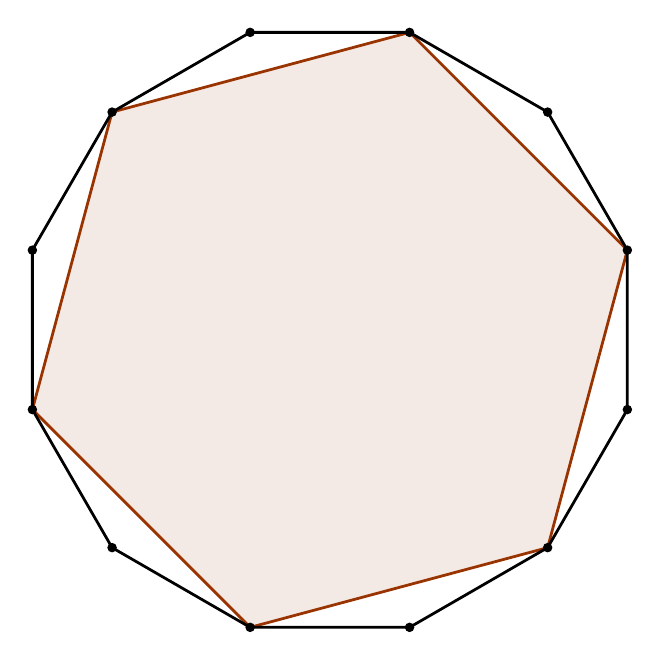
\begin{tikzpicture}[scale=.75]
\tkzSetUpLine[line width=1pt,color=black]
\tkzSetUpPoint[fill=black]

\tkzDefPoints{0/0/P0,2.7/0/P1}

\tkzDefRegPolygon[side,sides=12](P0,P1)

\tkzFillPolygon[fill=white](P1,P2,P3,P4,P5,P6,P7,P8,P9,P10,P11,P12)
\tkzFillPolygon[fill=ShapeClr,fill opacity=0.1](P1,P3,P5,P7,P9,P11)

\tkzDrawPolygons[color=ShapeClr](P1,P3,P5,P7,P9,P11)

\tkzDrawPolygon[color=black](P1,P2,P3,P4,P5,P6,P7,P8,P9,P10,P11,P12)
\tkzDrawPoints[size=3](P1,P2,P3,P4,P5,P6,P7,P8,P9,P10,P11,P12)

\end{tikzpicture}

\end{document}
